\section{Definition und Begrifflichkeiten}

\subsection{Didaktische Simulatoren}
Um den Begriff (didaktischer) \textit{Simulator} zu definieren, muss zunächst das zugrundeliegende Konzept des \textit{Modells} betrachtet werden. White und Ingalls beschreiben ein Modell als eine vereinfachte Abstraktion der Realität, die durch die Auswahl des geeigneten Umfangs und Detaillierungsgrades die relevanten Eigenschaften eines Untersuchungsgegenstands abbildet. Modelle kommen insbesondere dann zum Einsatz, wenn das reale System zu komplex, zu unpraktisch oder zu kostenintensiv wäre, um es direkt zu untersuchen \parencites[S.~12]{white_introduction_2009}[S.~5]{banks_what_2008}.

Darauf aufbauend stellt die \textit{Simulation} ein Teilgebiet der Modellbildung dar. Unter Simulation versteht man die Durchführung von Experimenten mit einem Modell, das die wesentlichen Eigenschaften des zugrundeliegenden Systems nachahmt, um dessen Verhalten unter verschiedenen Bedingungen untersuchen zu können \parencites[S.~12]{white_introduction_2009}[S.~6]{banks_what_2008}.

Ein \textit{Simulator} schließlich ist das Werkzeug oder System -- meist in Form von Software --, das diese Simulationen ermöglicht. Er implementiert das Modell und bietet eine Benutzungsumgebung, in der Interaktionen und Experimente mit dem Modell durchgeführt werden können \parencite[S.~304f]{duran_what_2020}.

Die Definition des Begriffs \textit{Simulator} ist eindeutig abzugrenzen von der Bezeichnung \textit{Emulator}. Ein Emulator hingegen strebt eine möglichst detailgetreue Nachbildung eines Zielsystems an, sodass Software oder Peripheriegeräte, die für das Originalsystem entwickelt wurden, unverändert darauf ausgeführt werden können \parencite[S.~1683]{mcgregor_relationship_2002}.

Besonders im Kontext der Lehre kommen sogenannte \textit{didaktische Simulatoren} zum Einsatz. Diese unterscheiden sich von hochgradig präzisen Forschungs- oder Industriesimulatoren dadurch, dass sie in erster Linie auf Verständlichkeit, Visualisierung und Interaktivität ausgerichtet sind. Ziel ist nicht die vollständige, detailgetreue Nachbildung eines Systems, sondern die Förderung von Lernprozessen durch eine für die Lernenden zugängliche Abstraktion komplexer Sachverhalte \parencites[S.~256]{muller_entwicklung_2020}[S.~1]{nystrom_teaching_2024}.

\subsection{Konzepte digitalen Lernens}

Da im Rahmen der Literaturrecherche verschiedene Konzepte des digitalen Lernens identifiziert wurden, werden diese nachfolgend kurz vorgestellt und im Hinblick auf ihre Relevanz für den Einsatz didaktischer Simulatoren erläutert.

\subsubsection{Organisationsformen des digitalen Lernens}

Digitale Medien und Technologien haben in den letzten Jahrzehnten eine Vielzahl an Lernformen hervorgebracht, die sich in Reichweite, Methodik und Grad der Individualisierung unterscheiden.

\sh{E-Learning}
Der Begriff \textit{E-Learning} dient als Oberbegriff für alle Formen des Lernens, die digitale Medien sowie Informations- und Kommunikationstechnologien zur Unterstützung oder Durchführung von Lehr- und Lernprozessen einsetzen. Dazu zählen sowohl webbasierte Kurse und Lernplattformen als auch multimediale Materialien wie Videos, interaktive Übungen oder Simulationen \parencite[S.~6]{kerres_mediendidaktik_2018}. Zentrale Merkmale des E-Learning sind die Orts- und Zeitunabhängigkeit, die Möglichkeit zur Interaktivität sowie der multimediale Charakter \parencite[S.~186f]{sanderson_e-learning_2002}. 

Andere Formen wie \textit{M-Learning} oder \textit{Blended Learning} stellen spezifische Ausprägungen dieses übergeordneten Begriffs dar \parencites[S.~74]{magenheim_blended_2003}[S.~3]{balaji_perspective_2016}.

\sh{M-Learning}
\textit{Mobile Learning} (kurz: M-Learning) wird in der Literatur häufig als eine Erweiterung bzw. neue Ausprägung des E-Learning verstanden, die durch den Einsatz mobiler Endgeräte wie Smartphones, Tablets, Notebooks oder PDAs über drahtlose Netzwerke ermöglicht wird \parencites[S.~3f]{balaji_perspective_2016}[S.~197]{basak_kumar_e-learning_2018}. 

M-Learning bezeichnet damit den Einsatz mobiler Technologien zur Unterstützung von Lernprozessen und kann als Schnittstelle zwischen Online-Lernen und mobiler Computertechnologie betrachtet werden \parencite[S.~265]{traxler_defining_2005}.

Während M-Learning also primär die technische Mobilität des Lernens hervorhebt, geht Blended Learning einen Schritt weiter und kombiniert digitale Formate mit klassischen Präsenzanteilen.

\sh{Blended Learning}
Blended Learning ist eine Lehr- und Lernform, die Methoden der Präsenzlehre mit Konzepten des E-Learning verbindet. Ziel ist die Förderung von Lernprozessen, in denen multimediale Materialien effektiv in individuelle und kooperative Lernphasen integriert werden können \parencite[S.~74]{magenheim_blended_2003}. Im deutschsprachigen Raum wird Blended Learning auch als \textit{hybrides Lernen} oder als \textit{vermischter Unterricht} bezeichnet \parencite[S.~29]{pfeffer_simulationsumgebungen_2008}.

In der Weiterentwicklung zu \textit{Blended Learning~2.0} werden klassische Präsenzformate noch stärker mit digitalen und hybriden Komponenten verknüpft. Charakteristisch ist hier der verstärkte Einsatz von Web~2.0-Technologien und sozialen Medien, wodurch flexible, personalisierbare Lernsettings entstehen, die sowohl selbstgesteuertes als auch kooperatives Lernen unterstützen \parencites{seufert_schulleitertagung_2014}{news_aktuell_gmbh_e-learning_2025}.

Während Blended Learning den Schwerpunkt auf die Integration von Präsenz- und Onlineformaten legt, stehen bei \ac{MOOC}s vollständig digitale, für eine große Zahl von Teilnehmenden offene Lernangebote im Vordergrund.

\sh{Massive Open Online Course (MOOC)}       
\textit{\ac{MOOC}s} sind internetbasierte Lehrveranstaltungen, die in der Regel für eine sehr große Zahl von Teilnehmenden konzipiert sind und ohne formale Zugangsbeschränkungen offen angeboten werden. Charakteristisch ist die Kombination aus multimedialen Inhalten, Online-Übungen, Diskussionsforen sowie Peer- oder Selbstbewertungen. Trotz der Offenheit verfolgen MOOCs einen strukturierten Lehrplan mit klar definierten Lernzielen \parencites[S.~5]{yuan_moocs_2013}[S.~204]{liyanagunawardena_moocs_2013}.

Während \ac{MOOC}s einen offenen, meist großskaligen Rahmen schaffen, fokussieren \ac{OER} stärker auf die Bereitstellung frei zugänglicher und wiederverwendbarer Lernmaterialien

\sh{Open Educational Resources (OER)}
\textit{\ac{OER}} bezeichnen Lehr- und Lernmaterialien, die sowohl frei zugänglich als auch offen lizenziert sind. Sie können ohne Kosten genutzt, angepasst und weiterverbreitet werden und eröffnen damit vielfältige Möglichkeiten zur gemeinsamen Gestaltung von Lernangeboten. Maßgeblich sind hierbei die sogenannten \enquote{5R-Rechte} (\textit{retain, reuse, revise, remix, redistribute}), die den Grad der Offenheit bestimmen \parencite[S.~134f]{wiley_defining_2018}.

\subsubsection{Lerntechnologien \& Umgebungen}

Neben didaktischen Konzepten spielt auch die technologische Entwicklung eine zentrale Rolle bei der Gestaltung digitaler Lernumgebungen. Neue Technologien eröffnen dabei nicht nur innovative Interaktionsmöglichkeiten, sondern auch datenbasierte Ansätze zur Analyse von Lernprozessen sowie virtuelle Räume, in denen praxisnahes Lernen ermöglicht wird.

\sh{Immersive Technologien}
\textit{Immersive Technologien} fassen Ansätze wie \ac{AR}, \ac{VR} und \ac{MR} zusammen, die es Lernenden ermöglichen, in digitale Umgebungen einzutauchen und dort interaktiv zu agieren. Häufig werden diese Technologien auch unter dem Oberbegriff \ac{XR} diskutiert \parencites[S.~82]{alnagrat_review_2022}[S.~256]{chen_information_2024}. In der Lehre finden immersive Technologien zunehmend Anwendung, da sie Motivation und Interaktivität fördern und hochgradig effektive Lernumgebungen schaffen können \parencite[S.~1]{izouaouen_education_2025}.

Während immersive Technologien in erster Linie auf die Gestaltung neuer Interaktionsformen abzielen, verfolgt Learning Analytics einen datengetriebenen Ansatz, um Lernprozesse zu erfassen und gezielt zu optimieren.

\sh{Learning Analytics}
\textit{Learning Analytics} bezeichnet die Erfassung, Sammlung, Analyse und Berichterstattung von Daten über Lernende und deren Kontexte mit dem Ziel, Lernprozesse sowie die Lernumgebungen, in denen sie stattfinden, besser zu verstehen und zu optimieren. Besondere Potenziale ergeben sich aus der Aufdeckung bislang verborgener Informationen in den Daten sowie aus deren gezielter Nutzung, etwa für didaktische Interventionen oder zur Vorhersage von Lernverläufen \parencite[S.~294]{xiao_applying_2019}.

Ergänzend zu diesen Ansätzen bieten virtuelle Labore konkrete Umgebungen, in denen Lernende Wissen anwenden und experimentell vertiefen können – oftmals unter Einsatz sowohl immersiver Technologien als auch von Learning-Analytics-Methoden.

\sh{Virtual Labs}
\textit{Virtuelle Labs} sind computerbasierte, interaktive Umgebungen, die es ermöglichen, Aufgaben auszuführen, die normalerweise in einem physischen Labor stattfinden würden. Über entsprechende Benutzeroberflächen können Simulationen, Animationen und teilweise sogar die Fernsteuerung realer Laborhardware erfolgen. Zahlreiche Studien haben den Einsatz virtueller Labore als Lehr- und Lerninstrument untersucht und ihre Wirksamkeit in nahezu allen Fällen bestätigt \parencite[S.~117]{achuthan_value_2011}.

In den letzten Jahren haben sich virtuelle Labore und Remote-Experimente durch Fortschritte in Webtechnologien und Anwendungen weiterentwickelt. Ziel ist es, die Erfahrungen eines klassischen Präsenzlabors möglichst realitätsnah abzubilden und dabei einen vergleichbaren Grad an Zugriff, Funktionalität und Flexibilität zu gewährleisten. Der Einsatz von virtuellen Welten und Mixed-Reality-Technologien eröffnet zudem neue Möglichkeiten für kollaboratives Arbeiten in immersiven 3D-Umgebungen, in denen Lernende komplexe Simulationen und Datensätze interaktiv erkunden und visualisieren können \parencite[S.~1]{savin-baden_understanding_2012}.

\subsubsection{Didaktische Konzepte zur Motivation}

Zur Förderung von Motivation und Engagement im Lernprozess haben sich in der Literatur verschiedene Konzepte etabliert, die spielerische Elemente auf unterschiedliche Weise nutzen. Die zentralen Ansätze sind Gamification, Gamified Learning und Game-Based Learning. Sie unterscheiden sich darin, ob Spielelemente lediglich in bestehende Lernumgebungen integriert werden oder ob das Spiel selbst den didaktischen Kern bildet.

\sh{Gamification}
\textit{Gamification} bezeichnet den Ansatz, Designelemente aus (Video-)Spielen in nicht-spielerische Kontexte zu übertragen \parencites[S.~2]{deterding_gamification_2011}[S.~9]{kapp_gamification_2012}. Durch den Einsatz solcher Spielelemente sollen Lernprozesse attraktiver gestaltet und Motivation sowie kognitives Engagement gefördert werden. Ein höheres Maß an Involviertheit kann dabei aus hochschuldidaktischer Sicht zu einem aktiveren und nachhaltigeren Lernen führen \parencites[S.~97ff]{chi_active-constructive-interactive_2009}[S.~1821]{chi_translating_2018}.

Der Begriff Gamification geht auf den Software-Entwickler Nick Pelling zurück, der Anfang der 2000er Jahre eine spieleähnliche Benutzeroberfläche für Bank- und Verkaufsautomaten entwarf \parencites{pelling_short_2011}[S.~2f]{deterding_gamification_2011}. In den folgenden Jahren haben sich neben Gamification auch verwandte Konzepte wie \textit{gamefulness}, \textit{gameful design} oder \textit{playful interaction design} etabliert, die sich teilweise überschneiden, jedoch unterschiedliche Akzentuierungen aufweisen \parencite[S.~2f]{deterding_gamification_2011}. Deterding et al. (2011) haben eine weit verbreitete Definition geprägt, die das Spiel als konstitutive Einheit betont und es von der allgemeinen Spielfreude (\textit{playfulness}) abgrenzt \parencites[S.~2f]{deterding_gamification_2011}[S.~452f]{schlag_gamifizierung_2021}.

Zu den typischen Gestaltungselementen der Gamification zählen unter anderem Punktesysteme, Ranglisten, Abzeichen, Belohnungen und Fortschrittsanzeigen. Sie sollen Lernende motivieren, indem sie Leistung sichtbar machen und Anreize zur weiteren Beschäftigung mit den Inhalten schaffen. Da sich die Spieleindustrie sowie die Anwendungsszenarien im Bildungsbereich kontinuierlich verändern, ist die Auswahl möglicher Spielelemente jedoch nicht abschließend festgelegt, sondern unterliegt einem dynamischen Wandel \parencite[S.~2f]{hamari_does_2014}.

Während Gamification also vor allem die Übertragung einzelner Spielelemente in nicht-spielerische Kontexte beschreibt, geht Gamified Learning einen Schritt weiter und rückt das didaktische Gesamtdesign in den Vordergrund.

\sh{Gamifiee Learning}
Unter \textit{Gamified Learning} wird der gezielte Einsatz von
Spielelementen in Lehr- und Lernszenarien verstanden, wobei der
didaktische Rahmen im Vordergrund steht. Die Theorie des
gamifizierten Lernens beschreibt dieses Zusammenspiel anhand
mehrerer Dimensionen: der Instruktion selbst, den Einstellungen
und Verhaltensweisen der Lernenden, den eingesetzten Spielelementen
sowie dem daraus resultierenden Lernerfolg \parencites[S.~6f]{landers_developing_2014}[S.~453]{schlag_gamifizierung_2021}.

Gamification kann dabei auf zwei Wegen wirken: Einerseits kann das
Verhalten der Lernenden die Wirksamkeit der Instruktion verstärken
oder abschwächen (moderierender Effekt). Andererseits können die
durch Spielelemente angestoßenen Einstellungen und Verhaltensweisen
selbst zum Lernerfolg beitragen (mediierender Effekt) \parencites[S.~6f]{landers_developing_2014}[S.~453]{schlag_gamifizierung_2021}.

Damit Gamified Learning erfolgreich ist, müssen Spielelemente also
so gestaltet werden, dass sie lernförderliche Verhaltensweisen
hervorrufen und in ein didaktisch sinnvolles Instruktionsdesign
eingebettet sind \parencites[S.~6f]{landers_developing_2014}[S.~453]{schlag_gamifizierung_2021}.

Im Gegensatz zu Gamification und Gamified Learning, bei denen Spielelemente in bestehende Lernumgebungen integriert werden, steht beim Game-Based Learning das Spiel selbst im Zentrum des didaktischen Prozesses.

\sh{Game-Based Learning}
\textit{Game-Based Learning} bezeichnet den Einsatz von digitalen
Spielen mit didaktischer Zielsetzung im Lehr- und Lernkontext. Im
deutschsprachigen Raum wird hierfür häufig auch der Begriff
\textit{Serious Games} verwendet, womit digitale, multimediale Spiele
gemeint sind, die nicht primär der Unterhaltung dienen, sondern einen
\enquote{ernsthaften} Hintergrund verfolgen \parencite[S.~14]{niegemann_kompendium_2008}.

\subsubsection{Individuelle \& adaptive Lernformen}

Im Kontext digitaler Lehre gewinnen Konzepte zunehmend an Bedeutung, die Lernprozesse stärker an die individuellen Voraussetzungen, Bedürfnisse und Ziele der Lernenden anpassen. Zu diesen zählen Ansätze wie Microlearning, Adaptive Learning und Personalized Learning, die eine inhaltliche oder methodische Individualisierung anstreben, sowie Collaborative Learning, das den sozialen Austausch als wichtigen Bestandteil des Lernprozesses hervorhebt.

\sh{Microlearning}
\textit{Microlearning} bezeichnet eine Form des digitalen Lernens, bei der Inhalte in kleine, leicht verdauliche Einheiten segmentiert werden. Ziel ist es, Lernenden einen schnellen und fokussierten Zugriff auf Wissen zu ermöglichen, der sich flexibel in ihren Alltag integrieren lässt. Typische Merkmale sind die Kürze der Lerneinheiten, ihre thematische Fokussierung sowie die Möglichkeit, sie in unterschiedlichen Kontexten, etwa mobil oder \enquote{on demand}, zu nutzen \parencite[S.~74]{chong_mvr-cls_2022}.

Ein sogenannter \textit{Microlearning Service} beschreibt, wie solche Lernressourcen systematisch bereitgestellt und an die individuellen Interessen der Lernenden angepasst werden können. Dieser Prozess umfasst drei wesentliche Schritte: (1) die Segmentierung von Inhalten in kleine Lerneinheiten, (2) die Annotation dieser Einheiten mit Metadaten und (3) die Empfehlung passender Inhalte an die jeweiligen Nutzerinnen und Nutzer \parencite[S.~152--154]{lin_survey_2019}.

Während Microlearning vor allem durch die Reduktion und Flexibilisierung von Lerninhalten geprägt ist, gehen adaptive Lernsysteme einen Schritt weiter, indem sie Inhalte dynamisch an den aktuellen Wissensstand anpassen.

\sh{Adaptive Learning}
\textit{Adaptive Learning} bezeichnet Lernsysteme, die Inhalte, Aufgaben und Lernpfade automatisch an die individuellen Bedürfnisse der Lernenden anpassen. Grundlage ist in der Regel eine Diagnose des aktuellen Wissensstandes sowie relevanter Lernmerkmale, auf deren Basis das System Schwierigkeitsgrad, Reihenfolge und Auswahl der Lerninhalte dynamisch steuert. Ergänzt wird dies durch kontinuierliches Feedback und eine laufende Anpassung des Lernprozesses, sodass Lernende dort abgeholt werden, wo sie stehen, und in ihrem individuellen Tempo gefördert werden können. Ziel adaptiver Lernsysteme ist es, Lernumgebungen effizienter, personalisierter und motivierender zu gestalten \parencite[S.~448]{zhao_research_2019}.

Während Adaptive Learning vor allem die technologische Umsetzung individueller Anpassungen in den Blick nimmt, verfolgt Personalized Learning einen umfassenderen Ansatz, der auch didaktische und organisatorische Aspekte einschließt.

\sh{Personalized Learning}
\textit{Personalized Learning} bezeichnet Lehr- und Lernformen, die sich stark an den individuellen Bedürfnissen, Interessen und Zielen der Lernenden orientieren. Im Vordergrund steht dabei die Anpassung von Lerninhalten, Methoden und Lernwegen an persönliche Voraussetzungen, Stärken und Schwächen. Während adaptive Systeme eine technologische Umsetzung dieser Idee ermöglichen, umfasst personalisiertes Lernen darüber hinaus auch didaktische und organisatorische Maßnahmen, etwa die Möglichkeit zur Wahl von Lernpfaden, zur Anpassung des Lerntempos oder zur Bearbeitung individueller Projekte. Ziel ist es, Lernumgebungen zu schaffen, die Motivation, Selbststeuerung und nachhaltigen Lernerfolg fördern \parencites[S.~6ff]{pane_informing_2017}[S.~2f]{gunawardena_personalized_2024}[S.~236--239]{walkington_appraising_2020}.

Neben diesen auf Individualisierung ausgerichteten Konzepten betont \textit{Collaborative Learning} den Wert gemeinsamer Interaktion und Wissenskonstruktion.

\sh{Collaborative Learning}
\textit{Collaborative Learning} bezeichnet eine Lehr- und Lernmethode, bei der Lernende gemeinsam an Aufgaben oder Problemstellungen arbeiten und ihr Wissen aktiv miteinander austauschen. Im Vordergrund steht nicht nur der individuelle Lernerfolg, sondern auch die gemeinsame Verantwortung innerhalb der Gruppe sowie die gegenseitige Unterstützung. Durch Diskussion, Interaktion und Kooperation wird Wissen nicht nur reproduziert, sondern gemeinsam konstruiert, wodurch sowohl kognitive als auch soziale Kompetenzen wie Kommunikation, Teamfähigkeit und Verantwortungsbewusstsein gefördert werden \parencite[S.~486]{laal_benefits_2021}.

\subsection{Lernpsychologische Grundlagen}

\subsubsection{Behaviorismus}

Der Behaviorismus versteht Lernen als eine Veränderung im beobachtbaren Verhalten, die durch Erfahrungen mit der Umwelt hervorgerufen wird. Zentrale Mechanismen sind die klassische und die operante Konditionierung \parencite[S.~15]{pfeiffer_simulationsumgebungen_2008}.

Die \textit{klassische Konditionierung}, die auf Pawlow zurückgeht, beschreibt Lernprozesse, bei denen ein ursprünglich neutraler Stimulus durch wiederholte Kopplung mit einem unkonditionierten Stimulus die Fähigkeit erlangt, dieselbe Reaktion auszulösen wie der unkonditionierte Stimulus selbst. Ein bekanntes Beispiel ist Pawlows Experiment mit Hunden, bei dem ein Glockenton (neutraler Stimulus) mit der Darbietung von Futter (unkonditionierter Stimulus) kombiniert wurde, sodass schließlich allein der Ton eine Speichelreaktion hervorrief \parencite[S.~7--10]{furstenau_lehr-lern-theorien_2019}.

Die \textit{operante Konditionierung}, entwickelt von Skinner, knüpft an Thorndikes \textit{Law of Effect} an, das besagt, dass Verhaltensweisen, die zu befriedigenden Konsequenzen führen, mit höherer Wahrscheinlichkeit erneut gezeigt werden. Im Zentrum steht hier die Beziehung zwischen Verhalten und Konsequenzen: Folgt auf ein Verhalten eine Verstärkung, steigt die Wahrscheinlichkeit, dass es unter ähnlichen Bedingungen wiederholt wird. Skinner unterscheidet dabei zwischen respondenten Verhaltensweisen, die durch einen Stimulus ausgelöst werden, und operanten Verhaltensweisen, die aktiv auf die Umwelt einwirken. Während klassische Konditionierung das Erlernen respondenten Verhaltens erklärt, bezieht sich die operante Konditionierung auf die Steuerung und Veränderung operanten Verhaltens \parencite[S.~15--17]{furstenau_lehr-lern-theorien_2019}.

\subsubsection{Kognitivismus}

Der Kognitivismus versteht Lernen wiederum als einen Prozess der aktiven Informationsaufnahme, -verarbeitung und -speicherung. Unter Kognition werden sämtliche \enquote{Prozesse des Wissens} verstanden, darunter Denken, Erinnerung, Sprache, Kreativität und Wahrnehmung. Lernende gelten in dieser Perspektive nicht als passiv durch äußere Reize gesteuert, sondern als aktive Individuen, die Informationen selbstständig verarbeiten und in bestehende Wissensstrukturen integrieren \parencite[S.~1]{furstenau_lehr-lern-theorien_2019}.

\begin{figure}[htbp]
    \centering
    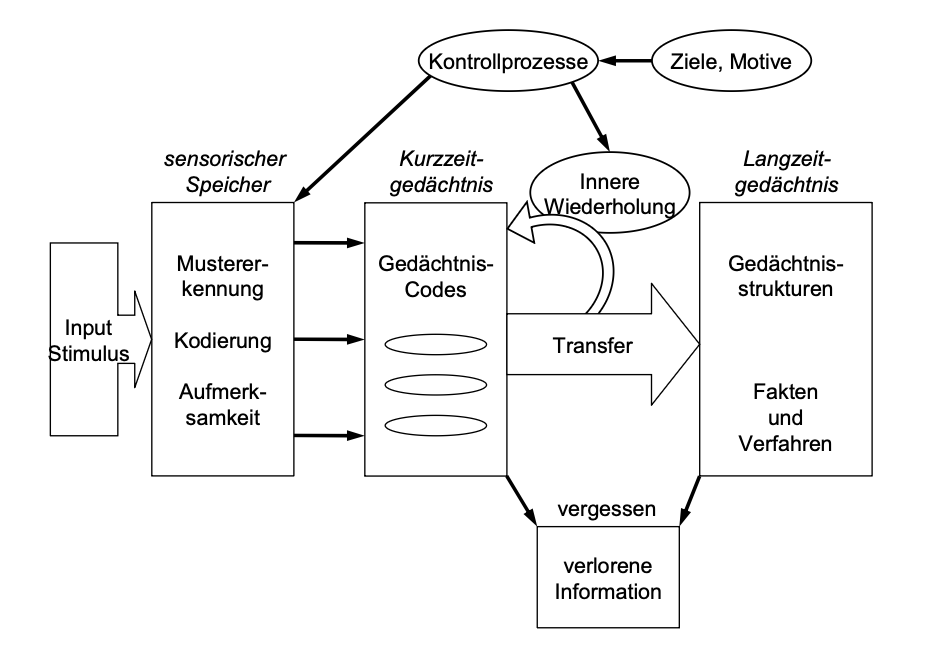
\includegraphics[width=0.90\textwidth]{img/Computermodell.png}
    \caption{Computermodell von Bower \& Hildgard }
	\parencite[S.~234]{bower_theorie_1984}
    \label{fig:computermodell}
\end{figure}

Eine wichtige Grundlage bildet das Computermodell von Bower \& Hilgard, das die menschliche Informationsverarbeitung analog zu einem Informationssystem beschreibt (siehe Abb.~\ref{fig:computermodell}). Hierbei werden eingehende Reize zunächst sensorisch aufgenommen, im Arbeitsgedächtnis verarbeitet und schließlich im Langzeitgedächtnis gespeichert. Die Kapazität des Arbeitsgedächtnisses ist dabei sowohl zeitlich als auch räumlich begrenzt: Informationen verfallen ohne Wiederholung nach wenigen Sekunden und können nur in einer beschränkten Anzahl gleichzeitig präsent gehalten werden. Daraus ergibt sich die Notwendigkeit, Inhalte zu strukturieren und durch Prozesse wie \enquote{Chunking} mit Vorwissen zu verknüpfen \parencite[S.~15]{pfeiffer_simulationsumgebungen_2008}.

Eine der einflussreichsten Theorien des multimedialen Lernens innerhalb des kognitivistischen Paradigmas ist die \ac{CTML} von Mayer \parencite[S.~102--105]{mayer_multimedia_2001}. Sie basiert auf drei zentralen Annahmen:
\begin{enumerate}
	\item Informationen werden über getrennte Kanäle verarbeitet – einen visuellen und einen auditiven
	\item die Verarbeitungskapazität ist in beiden Kanälen begrenzt
	\item Lernen erfordert aktive kognitive Verarbeitung, bei der Lernende neue Informationen mit vorhandenem Wissen verknüpfen
\end{enumerate}

Ergänzend stützt sich die Theorie auf Paivios Dual-Coding-Theory \parencite[S.~102f]{paivia_dual_2006}, nach der verbale und nonverbale Informationen in getrennten, aber miteinander verknüpften Repräsentationssystemen verarbeitet werden \parencite[S.~66f]{furstenau_lehr-lern-theorien_2019}.

\subsubsection{Konstruktivismus}

- Realität nicht objektiv wahrgenommen werden kann, sondern von den BetrachterInnen konstruiert wird
- Realität wird demnach "als eine interaktive Konzeption verstanden, in der Beobachter und Beobachtetes gegenseitig und strukturell miteinander gekoppelt sind"
- Lernen funktioniert, indem Menschen ihr Wissen konstruieren. Dies geschieht in Interaktion mit der aktuellen Lebenssituation udn dem früher erworbenen Wissen
- Unterschied zum Kognitivismus ist, dass beim Konstruktivismus nicht "das Lösen bereits präsenter Probleme im Vordergrund steht, sondern das eigenständige Generieren von Problemen"
- drei Lehransätze:
    - Cognitive Apprenticeshio
	- Knowledge Communities
	- Cognitive Tools

\sh{Erfahrungsbasierte Lerntheorie}

\sh{Konnektivismus}

\sh{Multimediales Lernen}
Was unter multimedialem Lernen zu verstehen ist, variiert in Abhängigkeit von der zugrunde liegenden Lerntheorie, die behavioristisch, kognitivistisch oder konstruktivistisch geprägt sein kann. \ Lernen als Reaktionsverstärkung : Bei dieser behavioristisch geprägten Art multimedialen Lernens besteht das Ziel darin, bestimmte Verbindungen im Gehirn zunächst aufzubauen und dann durch regelmäßiges Üben zu stärken. Beispiele für multimediale Lernumgebungen, die sich an diesem Lernverständnis orientieren, sind Lernprogramme zum 10-Finger-Schreiben oder so genannte Vokabeltrainer. Die Aufgabe des Lehrenden bzw. des Lernprogramms besteht ausschließlich darin, die richtigen Vokabelpaare zu präsentieren und abzufragen sowie richtige Antworten zu belohnen bzw. falsche zu bestrafen (z. B. indem die Lektion erneut bearbeitet werden muss). \ Lernen als Informationserwerb bzw. -verarbeitung : Dieses eher kognitivistisch geprägte Verständnis geht davon aus, dass beim Lernen neue Informationen aufgenommen und zur bestehenden Wissensbasis hinzugefügt werden. Die zu lernenden Informationen werden durch die multimediale Lernumgebung bereitgestellt. Dies kann beispielsweise durch das Aufrufen geeigneter Internetseiten geschehen. 2 \ Lernen als aktive Wissenskonstruktion : Neuere lernpsychologische Forschung hat gezeigt, dass Lernende neue Informationen keineswegs wie ein Schwamm einfach „aufsaugen“, sondern, dass sie diese Informationen vor dem Hintergrund ihres existierenden Vorwissens interpretieren ( Mayer , 2009, S. 14 – 19). Die Lernenden konstruieren ihr Wissen selbstständig (Kapitel 5 in diesem Buch). Dieser Auffassung zufolge geschieht multimediales Lernen immer dann, wenn aufgrund der gemeinsamen Darbietung von Worten und Bildern mentale Repräsentationen aufgebaut oder modifiziert werden ( Mayer , 2005b, S. 15).
